\documentclass[10pt,a4paper]{article}
\usepackage[utf8]{inputenc}
\usepackage{amsmath}
\usepackage{amsfonts}
\usepackage{amssymb}
\usepackage{graphicx}

\title{Exercise 1}
\author{Sean Fortuna - 2011-18128}
\date{}


\newcommand{\deri}[2]{\dfrac{\textnormal{d} #1 }{\textnormal{d} #2}}

\newcommand{\topic}{\vspace{-1mm} \noindent \rule{0.5\textwidth}{0.4pt}  \vspace{1mm}}
\begin{document}
\maketitle

Given two modes of the same infection, whereby one infection $I_1$ is more infectious than the other infection of the same kind $I_2$ (different $\beta$ values), provide the following
\begin{enumerate}
\item Compartmental flow diagram of the dynamics (write the assumptions).
\item Stoichiometric equation for each conversion.
\item Corresponding differential equation for the system (well-mixed assumption).
\end{enumerate}

\topic
We consider the following compartmental flow diagram:
\begin{center}
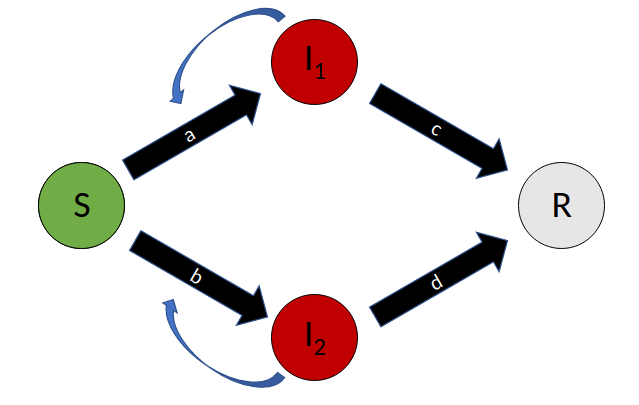
\includegraphics[width=0.5\textwidth]{model.png} 
\end{center}
We assume that the susceptible population may only become infected by one of the two types of infections, and that this transformation from susceptible to infected is promoted by the population infected with the corresponding infection type. That is, only the population infected with $I_1$ may induce a susceptible person to become infected with $I_1$. \\

After infection, each infected population spontaneously becomes recovered at some rate proportional to the size of the population infected with that type of disease.

\topic

We refer to the labelling of the arrows, and define the related stoichiometric equation.
\begin{equation}
\begin{array}{ccc}
\textrm{a}&:& S^* + I_1 \to I_1^* + I_1 \\
\textrm{b}&:& S^* + I_2 \to I_2^* + I_2 \\
\textrm{c}&:& I_1 \to R \\
\textrm{d}&:& I_2 \to R
\end{array}
\end{equation}

\topic

Let the total population be $N$, and let the population of susceptible, infected with $I_1$, infected with $I_2$ and recovered by denoted by $N_S$, $N_{I_1}$, $N_{I_2}$ and $N_R$ respectively. They must satisfy
\begin{equation}
N = N_S + N_{I_1} + N_{I_2} + N_R.
\end{equation}
We may define number densities,
\begin{equation}
1 = \dfrac{N_S + N_{I_1} + N_{I_2} + N_R}{N} = n_S + n_{I_1} + n_{I_2} + n_R
\end{equation}
Note that this implies that
\begin{equation}
\deri{}{t} \left( n_S + n_{I_1} + n_{I_2} + n_R \right) = 0
\label{eq:conservation}
\end{equation}
In a well-mixed population, the rate at which a certain reaction proceeds is given by the probability of the reactants of finding each other.
\begin{equation}
\begin{array}{ccccc}
\textrm{a}&:& S^* + I_1 \to I_1^* + I_1 &\to& \sim n_s \cdot n_{I_1} \\
\textrm{b}&:& S^* + I_2 \to I_2^* + I_2 &\to& \sim n_s \cdot n_{I_2} \\
\textrm{c}&:& I_1 \to R &\to& \sim n_{I_1}\\
\textrm{d}&:& I_2 \to R & \to& \sim n_{I_2}
\end{array}
\end{equation}

By the assumptions of the problem, we assume that $a$ proceeds faster than $b$ and that $c$ and $d$ proceed at an equal rate keeping all things equal. \\

We arrive at the following differential equations
\begin{eqnarray}
\deri{n_S}{t} &=& - \beta_1 n_S \cdot n_{I_1} - \beta_2 n_S \cdot n_{I_2} \\
\deri{n_{I_1}}{t} &=& \beta_1 n_S \cdot n_{I_1} - \alpha n_{I_1} \\
\deri{n_{I_2}}{t} &=& \beta_2 n_S \cdot n_{I_2} - \alpha n_{I_2} \\
\deri{n_R}{t} &=& \alpha n_{I_1} + \alpha n_{I_2}
\end{eqnarray}
where
\begin{equation}
\beta_1 > \beta_2 > 0, \qquad \alpha > 0.
\end{equation}
We note that the quantities must be strictly greater than 0. For $\beta$, this means that the diseases are communicable. For $\alpha$, this just means that, one way or another, an infected person becomes `recovered' (or perhaps removed or something else). \\

As a final check, it is easy to show that the differential equations satisfy the conservation property \eqref{eq:conservation}.

\end{document}